%% Beginning of file 'sample631.tex'
%%
%% Modified 2022 May  
%%
%% This is a sample manuscript marked up using the
%% AASTeX v6.31 LaTeX 2e macros.
%%
%% AASTeX is now based on Alexey Vikhlinin's emulateapj.cls 
%% (Copyright 2000-2015).  See the classfile for details.

%% AASTeX requires revtex4-1.cls and other external packages such as
%% latexsym, graphicx, amssymb, longtable, and epsf.  Note that as of 
%% Oct 2020, APS now uses revtex4.2e for its journals but remember that 
%% AASTeX v6+ still uses v4.1. All of these external packages should 
%% already be present in the modern TeX distributions but not always.
%% For example, revtex4.1 seems to be missing in the linux version of
%% TexLive 2020. One should be able to get all packages from www.ctan.org.
%% In particular, revtex v4.1 can be found at 
%% https://www.ctan.org/pkg/revtex4-1.

%% The first piece of markup in an AASTeX v6.x document is the \documentclass
%% command. LaTeX will ignore any data that comes before this command. The 
%% documentclass can take an optional argument to modify the output style.
%% The command below calls the preprint style which will produce a tightly 
%% typeset, one-column, single-spaced document.  It is the default and thus
%% does not need to be explicitly stated.
%%
%% using aastex version 6.3
%%\documentclass[linenumbers]{aastex631}

%%\documentclass{aastex631}

%% The default is a single spaced, 10 point font, single spaced article.
%% There are 5 other style options available via an optional argument. They
%% can be invoked like this:
%%
%% \documentclass[arguments]{aastex631}

\documentclass[manuscript]{aastex631}
\usepackage{graphicx} % for including images
\usepackage{subcaption} % for subfigures

% Remove paragraph indentation
\setlength{\parindent}{0pt}

%% 
%% where the layout options are:
%%
%%  twocolumn   : two text columns, 10 point font, single spaced article.
%%                This is the most compact and represent the final published
%%                derived PDF copy of the accepted manuscript from the publisher
%%  manuscript  : one text column, 12 point font, double spaced article.
%%  preprint    : one text column, 12 point font, single spaced article.  
%%  preprint2   : two text columns, 12 point font, single spaced article.
%%  modern      : a stylish, single text column, 12 point font, article with
%% 		  wider left and right margins. This uses the Daniel
%% 		  Foreman-Mackey and David Hogg design.
%%  RNAAS       : Supresses an abstract. Originally for RNAAS manuscripts 
%%                but now that abstracts are required this is obsolete for
%%                AAS Journals. Authors might need it for other reasons. DO NOT
%%                use \begin{abstract} and \end{abstract} with this style.
%%
%% Note that you can submit to the AAS Journals in any of these 6 styles.
%%
%% There are other optional arguments one can invoke to allow other stylistic
%% actions. The available options are:
%%
%%   astrosymb    : Loads Astrosymb font and define \astrocommands. 
%%   tighten      : Makes baselineskip slightly smaller, only works with 
%%                  the twocolumn substyle.
%%   times        : uses times font instead of the default
%%   linenumbers  : turn on lineno package.
%%   trackchanges : required to see the revision mark up and print its output
%%   longauthor   : Do not use the more compressed footnote style (default) for 
%%                  the author/collaboration/affiliations. Instead print all
%%                  affiliation information after each name. Creates a much 
%%                  longer author list but may be desirable for short 
%%                  author papers.
%% twocolappendix : make 2 column appendix.
%%   anonymous    : Do not show the authors, affiliations and acknowledgments 
%%                  for dual anonymous review.
%%
%% these can be used in any combination, e.g.
%%
%% \documentclass[twocolumn,linenumbers,trackchanges]{aastex631}
%%
%% AASTeX v6.* now includes \hyperref support. While we have built in specific
%% defaults into the classfile you can manually override them with the
%% \hypersetup command. For example,
%%
%% \hypersetup{linkcolor=red,citecolor=green,filecolor=cyan,urlcolor=magenta}
%%
%% will change the color of the internal links to red, the links to the
%% bibliography to green, the file links to cyan, and the external links to
%% magenta. Additional information on \hyperref options can be found here:
%% https://www.tug.org/applications/hyperref/manual.html#x1-40003
%%
%% Note that in v6.3 "bookmarks" has been changed to "true" in hyperref
%% to improve the accessibility of the compiled pdf file.
%%
%% If you want to create your own macros, you can do so
%% using \newcommand. Your macros should appear before
%% the \begin{document} command.
%%
\newcommand{\vdag}{(v)^\dagger}
\newcommand\aastex{AAS\TeX}
\newcommand\latex{La\TeX}

%% Reintroduced the \received and \accepted commands from AASTeX v5.2
%\received{March 1, 2021}
%\revised{April 1, 2021}
%\accepted{\today}

%% Command to document which AAS Journal the manuscript was submitted to.
%% Adds "Submitted to " the argument.
%\submitjournal{PSJ}

%% For manuscript that include authors in collaborations, AASTeX v6.31
%% builds on the \collaboration command to allow greater freedom to 
%% keep the traditional author+affiliation information but only show
%% subsets. The \collaboration command now must appear AFTER the group
%% of authors in the collaboration and it takes TWO arguments. The last
%% is still the collaboration identifier. The text given in this
%% argument is what will be shown in the manuscript. The first argument
%% is the number of author above the \collaboration command to show with
%% the collaboration text. If there are authors that are not part of any
%% collaboration the \nocollaboration command is used. This command takes
%% one argument which is also the number of authors above to show. A
%% dashed line is shown to indicate no collaboration. This example manuscript
%% shows how these commands work to display specific set of authors 
%% on the front page.
%%
%% For manuscript without any need to use \collaboration the 
%% \AuthorCollaborationLimit command from v6.2 can still be used to 
%% show a subset of authors.
%
%\AuthorCollaborationLimit=2
%
%% will only show Schwarz & Muench on the front page of the manuscript
%% (assuming the \collaboration and \nocollaboration commands are
%% commented out).
%%
%% Note that all of the author will be shown in the published article.
%% This feature is meant to be used prior to acceptance to make the
%% front end of a long author article more manageable. Please do not use
%% this functionality for manuscripts with less than 20 authors. Conversely,
%% please do use this when the number of authors exceeds 40.
%%
%% Use \allauthors at the manuscript end to show the full author list.
%% This command should only be used with \AuthorCollaborationLimit is used.

%% The following command can be used to set the latex table counters.  It
%% is needed in this document because it uses a mix of latex tabular and
%% AASTeX deluxetables.  In general it should not be needed.
%\setcounter{table}{1}

%%%%%%%%%%%%%%%%%%%%%%%%%%%%%%%%%%%%%%%%%%%%%%%%%%%%%%%%%%%%%%%%%%%%%%%%%%%%%%%%
%%
%% The following section outlines numerous optional output that
%% can be displayed in the front matter or as running meta-data.
%%
%% If you wish, you may supply running head information, although
%% this information may be modified by the editorial offices.
%\shorttitle{AASTeX v6.3.1 Sample article}
%\shortauthors{Schwarz et al.}
%%
%% You can add a light gray and diagonal water-mark to the first page 
%% with this command:
%% \watermark{text}
%% where "text", e.g. DRAFT, is the text to appear.  If the text is 
%% long you can control the water-mark size with:
%% \setwatermarkfontsize{dimension}
%% where dimension is any recognized LaTeX dimension, e.g. pt, in, etc.
%%
%%%%%%%%%%%%%%%%%%%%%%%%%%%%%%%%%%%%%%%%%%%%%%%%%%%%%%%%%%%%%%%%%%%%%%%%%%%%%%%%
%\graphicspath{{./}{figures/}}


%% This is the end of the preamble.  Indicate the beginning of the
%% manuscript itself with \begin{document}.

\begin{document}

%%\title{Accessible Self-Checkout: Automating Fruit Recognition}

%% LaTeX will automatically break titles if they run longer than
%% one line. However, you may use \\ to force a line break if
%% you desire. In v6.31 you can include a footnote in the title.

%% A significant change from earlier AASTEX versions is in the structure for 
%% calling author and affiliations. The change was necessary to implement 
%% auto-indexing of affiliations which prior was a manual process that could 
%% easily be tedious in large author manuscripts.
%%
%% The \author command is the same as before except it now takes an optional
%% argument which is the 16 digit ORCID. The syntax is:
%% \author[xxxx-xxxx-xxxx-xxxx]{Author Name}
%%
%% This will hyperlink the author name to the author's ORCID page. Note that
%% during compilation, LaTeX will do some limited checking of the format of
%% the ID to make sure it is valid. If the "orcid-ID.png" image file is 
%% present or in the LaTeX pathway, the OrcID icon will appear next to
%% the authors name.
%%
%% Use \affiliation for affiliation information. The old \affil is now aliased
%% to \affiliation. AASTeX v6.31 will automatically index these in the header.
%% When a duplicate is found its index will be the same as its previous entry.
%%
%% Note that \altaffilmark and \altaffiltext have been removed and thus 
%% can not be used to document secondary affiliations. If they are used latex
%% will issue a specific error message and quit. Please use multiple 
%% \affiliation calls for to document more than one affiliation.
%%
%% The new \altaffiliation can be used to indicate some secondary information
%% such as fellowships. This command produces a non-numeric footnote that is
%% set away from the numeric \affiliation footnotes.  NOTE that if an
%% \altaffiliation command is used it must come BEFORE the \affiliation call,
%% right after the \author command, in order to place the footnotes in
%% the proper location.
%%
%% Use \email to set provide email addresses. Each \email will appear on its
%% own line so you can put multiple email address in one \email call. A new
%% \correspondingauthor command is available in V6.31 to identify the
%% corresponding author of the manuscript. It is the author's responsibility
%% to make sure this name is also in the author list.
%%
%% While authors can be grouped inside the same \author and \affiliation
%% commands it is better to have a single author for each. This allows for
%% one to exploit all the new benefits and should make book-keeping easier.
%%
%% If done correctly the peer review system will be able to
%% automatically put the author and affiliation information from the manuscript
%% and save the corresponding author the trouble of entering it by hand.

%\correspondingauthor{August Muench}
%\email{greg.schwarz@aas.org, gus.muench@aas.org}

\title{\vspace{-0.5cm}\large CEN/BMI 598: EMBEDDED MACHINE LEARNING\\\vspace{0.5em}Accessible Self-Checkout: Automating Fruit Recognition}
\author{
    Manish Kumar Peteri,
    Narain Pattabhiraman,
    Swathi Mengji.
    %%\textsuperscript{1}Arizona State University\\
}

%% Note that the \and command from previous versions of AASTeX is now
%% depreciated in this version as it is no longer necessary. AASTeX 
%% automatically takes care of all commas and "and"s between authors names.

%% AASTeX 6.31 has the new \collaboration and \nocollaboration commands to
%% provide the collaboration status of a group of authors. These commands 
%% can be used either before or after the list of corresponding authors. The
%% argument for \collaboration is the collaboration identifier. Authors are
%% encouraged to surround collaboration identifiers with ()s. The 
%% \nocollaboration command takes no argument and exists to indicate that
%% the nearby authors are not part of surrounding collaborations.

%% Mark off the abstract in the ``abstract'' environment. 
\begin{abstract}
% Remove paragraph indentation
\setlength{\parindent}{0pt}

In the realm of modern self-checkout systems within supermarkets, the manual input of fruit data emerges as a cumbersome and time-intensive process, presenting challenges for all shoppers and notably impacting individuals with visual impairments or blindness. In response to this challenge, our project harnesses the capabilities of the Raspberry Pi 3 B+ microprocessor alongside the 5MP wide-angle Raspberry Pi camera module version 1.0 to devise an innovative and inclusive self-checkout solution.

By incorporating the Raspberry Pi camera module, our system adeptly captures high-quality images of fruits, facilitating object and image identification. This image recognition process seamlessly integrates into the workflow of the self-checkout counter, alleviating the need for manual data input during the checkout process.

The crux of our project lies not only in streamlining the self-checkout experience for all shoppers but also in extending these benefits to individuals with visual impairments or blindness. Through leveraging advanced image recognition technologies, our solution fosters a more inclusive, efficient, and user-friendly retail environment. The intersection of cutting-edge hardware and software in our project represents a significant leap toward creating an accessible and equitable shopping experience for individuals of diverse abilities..

\vspace{200pt} 
\end{abstract}

%% Keywords should appear after the \end{abstract} command. 
%% The AAS Journals now uses Unified Astronomy Thesaurus concepts:
%% https://astrothesaurus.org
%% You will be asked to selected these concepts during the submission process
%% but this old "keyword" functionality is maintained in case authors want
%% to include these concepts in their preprints.
% \keywords{Classical Novae (251) --- Ultraviolet astronomy(1736) }

%% From the front matter, we move on to the body of the paper.
%% Sections are demarcated by \section and \subsection, respectively.
%% Observe the use of the LaTeX \label
%% command after the \subsection to give a symbolic KEY to the
%% subsection for cross-referencing in a \ref command.
%% You can use LaTeX's \ref and \label commands to keep track of
%% cross-references to sections, equations, tables, and figures.
%% That way, if you change the order of any elements, LaTeX will
%% automatically renumber them.
%%
%% We recommend that authors also use the natbib \citep
%% and \citet commands to identify citations.  The citations are
%% tied to the reference list via symbolic KEYs. The KEY corresponds
%% to the KEY in the \bibitem in the reference list below. 

\section{Introduction} \label{sec:intro}

Self-checkout counters have become an integral part of the modern supermarket experience, offering shoppers the convenience of a faster and more autonomous transaction process. However, the manual input of product information, especially when dealing with items such as fresh produce, can often be a daunting and time-consuming task. This challenge is exacerbated for individuals with visual impairments or blindness, who rely on assistance or costly specialized services to navigate the self-checkout process. In response to these concerns, our project introduces an innovative and inclusive solution that redefines the self-checkout experience.

The heart of our project is the utilization of cutting-edge technology, primarily the Raspberry pi 3b+ microprocessor and the Raspberry camera module V1.0, which seamlessly integrate into existing self-checkout systems.Furthermore, the integration of the Raspberry Pi camera module allows our system to capture high-resolution images of the fruit. Leveraging image classification and processing capabilities, our solution ensures accurate fruit identification, reducing the need for manual data entry and minimizing errors in the self-checkout process.

In keeping with our commitment to inclusivity, we have designed a user-friendly interface that can adapt to individual preferences. Shoppers have the option of receiving information through audio output or a visual display on an external device, making the self-checkout process accessible to everyone, regardless of their visual abilities.

In this context, our project not only streamlines the self-checkout experience for all shoppers but also extends its benefits to those with visual impairments or blindness. By providing an efficient, reliable, and inclusive self-checkout solution, we aim to create a more user-friendly and accessible retail environment, where technology serves as a bridge to a more convenient and inclusive shopping experience

\vspace{100pt} 

\section{Related Work} \label{sec:style}
Recent developments collectively aim to create more accurate, efficient, and user-friendly fruit and vegetable recognition solutions for self-checkout systems. As technology continues to evolve, the retail industry can expect further enhancements in this critical aspect of automated shopping. 

One such example is Vynamic Smart Vision. Diebold Nixdorf's Vynamic Smart Vision integrates SeeWare machine learning to recognize products without barcodes, including fruits, vegetables, and baked goods. This technology will be showcased at NRF's Big Show 2023 event in New York City.

KanduAI's Produce Recognition Technology eliminates the need for manually selecting non-barcoded items, particularly relevant for products like fresh produce. Their technology aims to enhance efficiency, improve security, and elevate the overall shopping experience. Retailers are encouraged to consider upgrading to these solutions to embrace the future of retail.

A potential solution to fully automate checkout without the need for barcodes relies on advanced machine image-recognition technology. While image recognition for pre-packaged products has seen significant progress, detecting fresh produce within semi-transparent plastic packaging poses a greater challenge due to the difficulty in obtaining accurate images through the plastic. 

In the "Optimization of existing MatchX Technology" project conducted for ITAB, a manufacturer of self-checkout technology, experts from Wageningen University & Research addressed this challenge. They employed near-infrared hyperspectral imaging in combination with spectral orthogonalization, a unique data-processing technique that effectively eliminates the interference of plastic packaging from the product images. This innovative approach was successfully tested and validated for three commonly consumed fruits: bananas, apples, and pears. The equipment demonstrated its capability to identify these fruits and accurately count them, even when they were enclosed in three different types of semi-transparent packaging commonly found in Dutch supermarkets—namely, low-density, intermediate-density, and high-density polyethylene.

\vspace{46pt} 

\section{System Design} \label{sec:cite}

\textbf{System Design:}

\begin{figure}[ht]
    \centering
    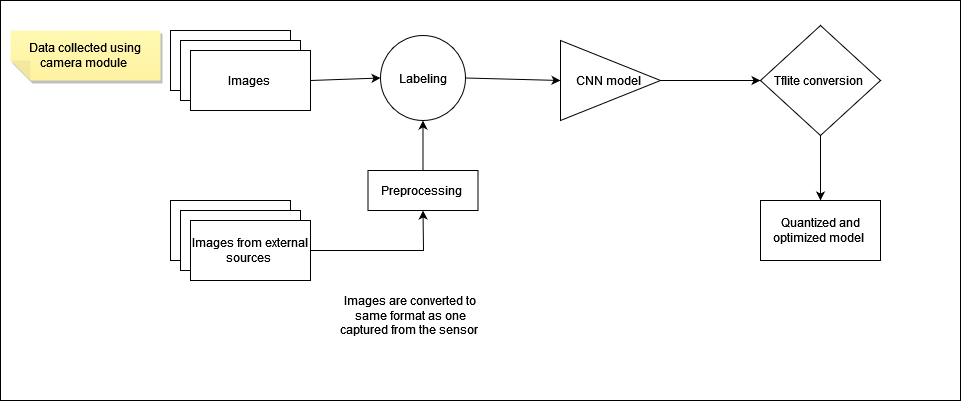
\includegraphics[width=1\linewidth]{EML project .drawio.png}
    \caption{System design for training the machine learning model}
    \label{fig:1}
\end{figure}

The system design of our automated fruit recognition involves the seamless integration of hardware components, sensor technology, and machine learning algorithms to create an efficient and inclusive self-checkout experience.

\vspace{12pt} 

\textbf{Hardware Components:}

\begin{itemize}
    \item \textbf{Raspberry Pi 3b+:}
    
The Raspberry Pi 3B+ is a compact and versatile single-board computer designed to provide a cost-effective platform for various computing projects. Powered by a quad-core ARM Cortex-A53 processor running at 1.4 GHz, coupled with 1GB of RAM, the Raspberry Pi 3B+ offers improved processing power and multitasking capabilities compared to its predecessors. Equipped with a set of GPIO (General Purpose Input/Output) pins, HDMI output, Ethernet port, four USB ports, and built-in Wi-Fi and Bluetooth capabilities, it facilitates seamless connectivity and interaction with a wide range of peripherals. Its support for microSD cards as the primary storage medium allows for scalable and customizable storage solutions. The Raspberry Pi 3B+ is commonly used in projects ranging from educational programming and hobbyist tinkering to more complex applications such as home automation, media centers, and Internet of Things (IoT) devices. Its open-source nature and a vibrant community contribute to its popularity, making it an accessible and powerful tool for enthusiasts and professionals alike.
    
    \item \textbf{Raspberry Pi 3b+ Camera Module:}
    
The Raspberry Pi Camera Module v1.0 is a compact imaging solution designed specifically for Raspberry Pi single-board computers. Developed by the Raspberry Pi Foundation, this camera module features a 5-megapixel fixed-focus camera sensor capable of capturing still images and video. The module connects to the Raspberry Pi through a dedicated camera interface (CSI) ribbon cable, ensuring a direct and efficient connection.

The camera module v1.0 has dimensions of 25mm x 20mm x 9mm, making it a small and lightweight accessory suitable for a wide range of applications. It supports video resolutions up to 1080p at 30 frames per second, providing clear and detailed footage. The fixed-focus lens simplifies usage, eliminating the need for manual adjustments, and the module is equipped with a small PCB with a camera sensor, making it easy to integrate into various projects.

Common applications of the Raspberry Pi Camera Module v1.0 include DIY photography and videography projects, surveillance systems, and educational purposes. The module is compatible with a variety of software and libraries, including the official Raspberry Pi Camera software, as well as popular platforms like OpenCV for image processing. Its affordability, ease of use, and direct integration with Raspberry Pi boards make it a popular choice for hobbyists and developers seeking a compact and capable imaging solution for their projects.
\end{itemize}

\textbf{Data Acquisition and Preprocessing:}

The Raspberry Pi 3b+ collects data from the camera module mounted on it. This data is crucial for obtaining metadata that enhances the identification process.

\begin{figure}[h]
    \centering
    \begin{subfigure}{0.3\textwidth}
        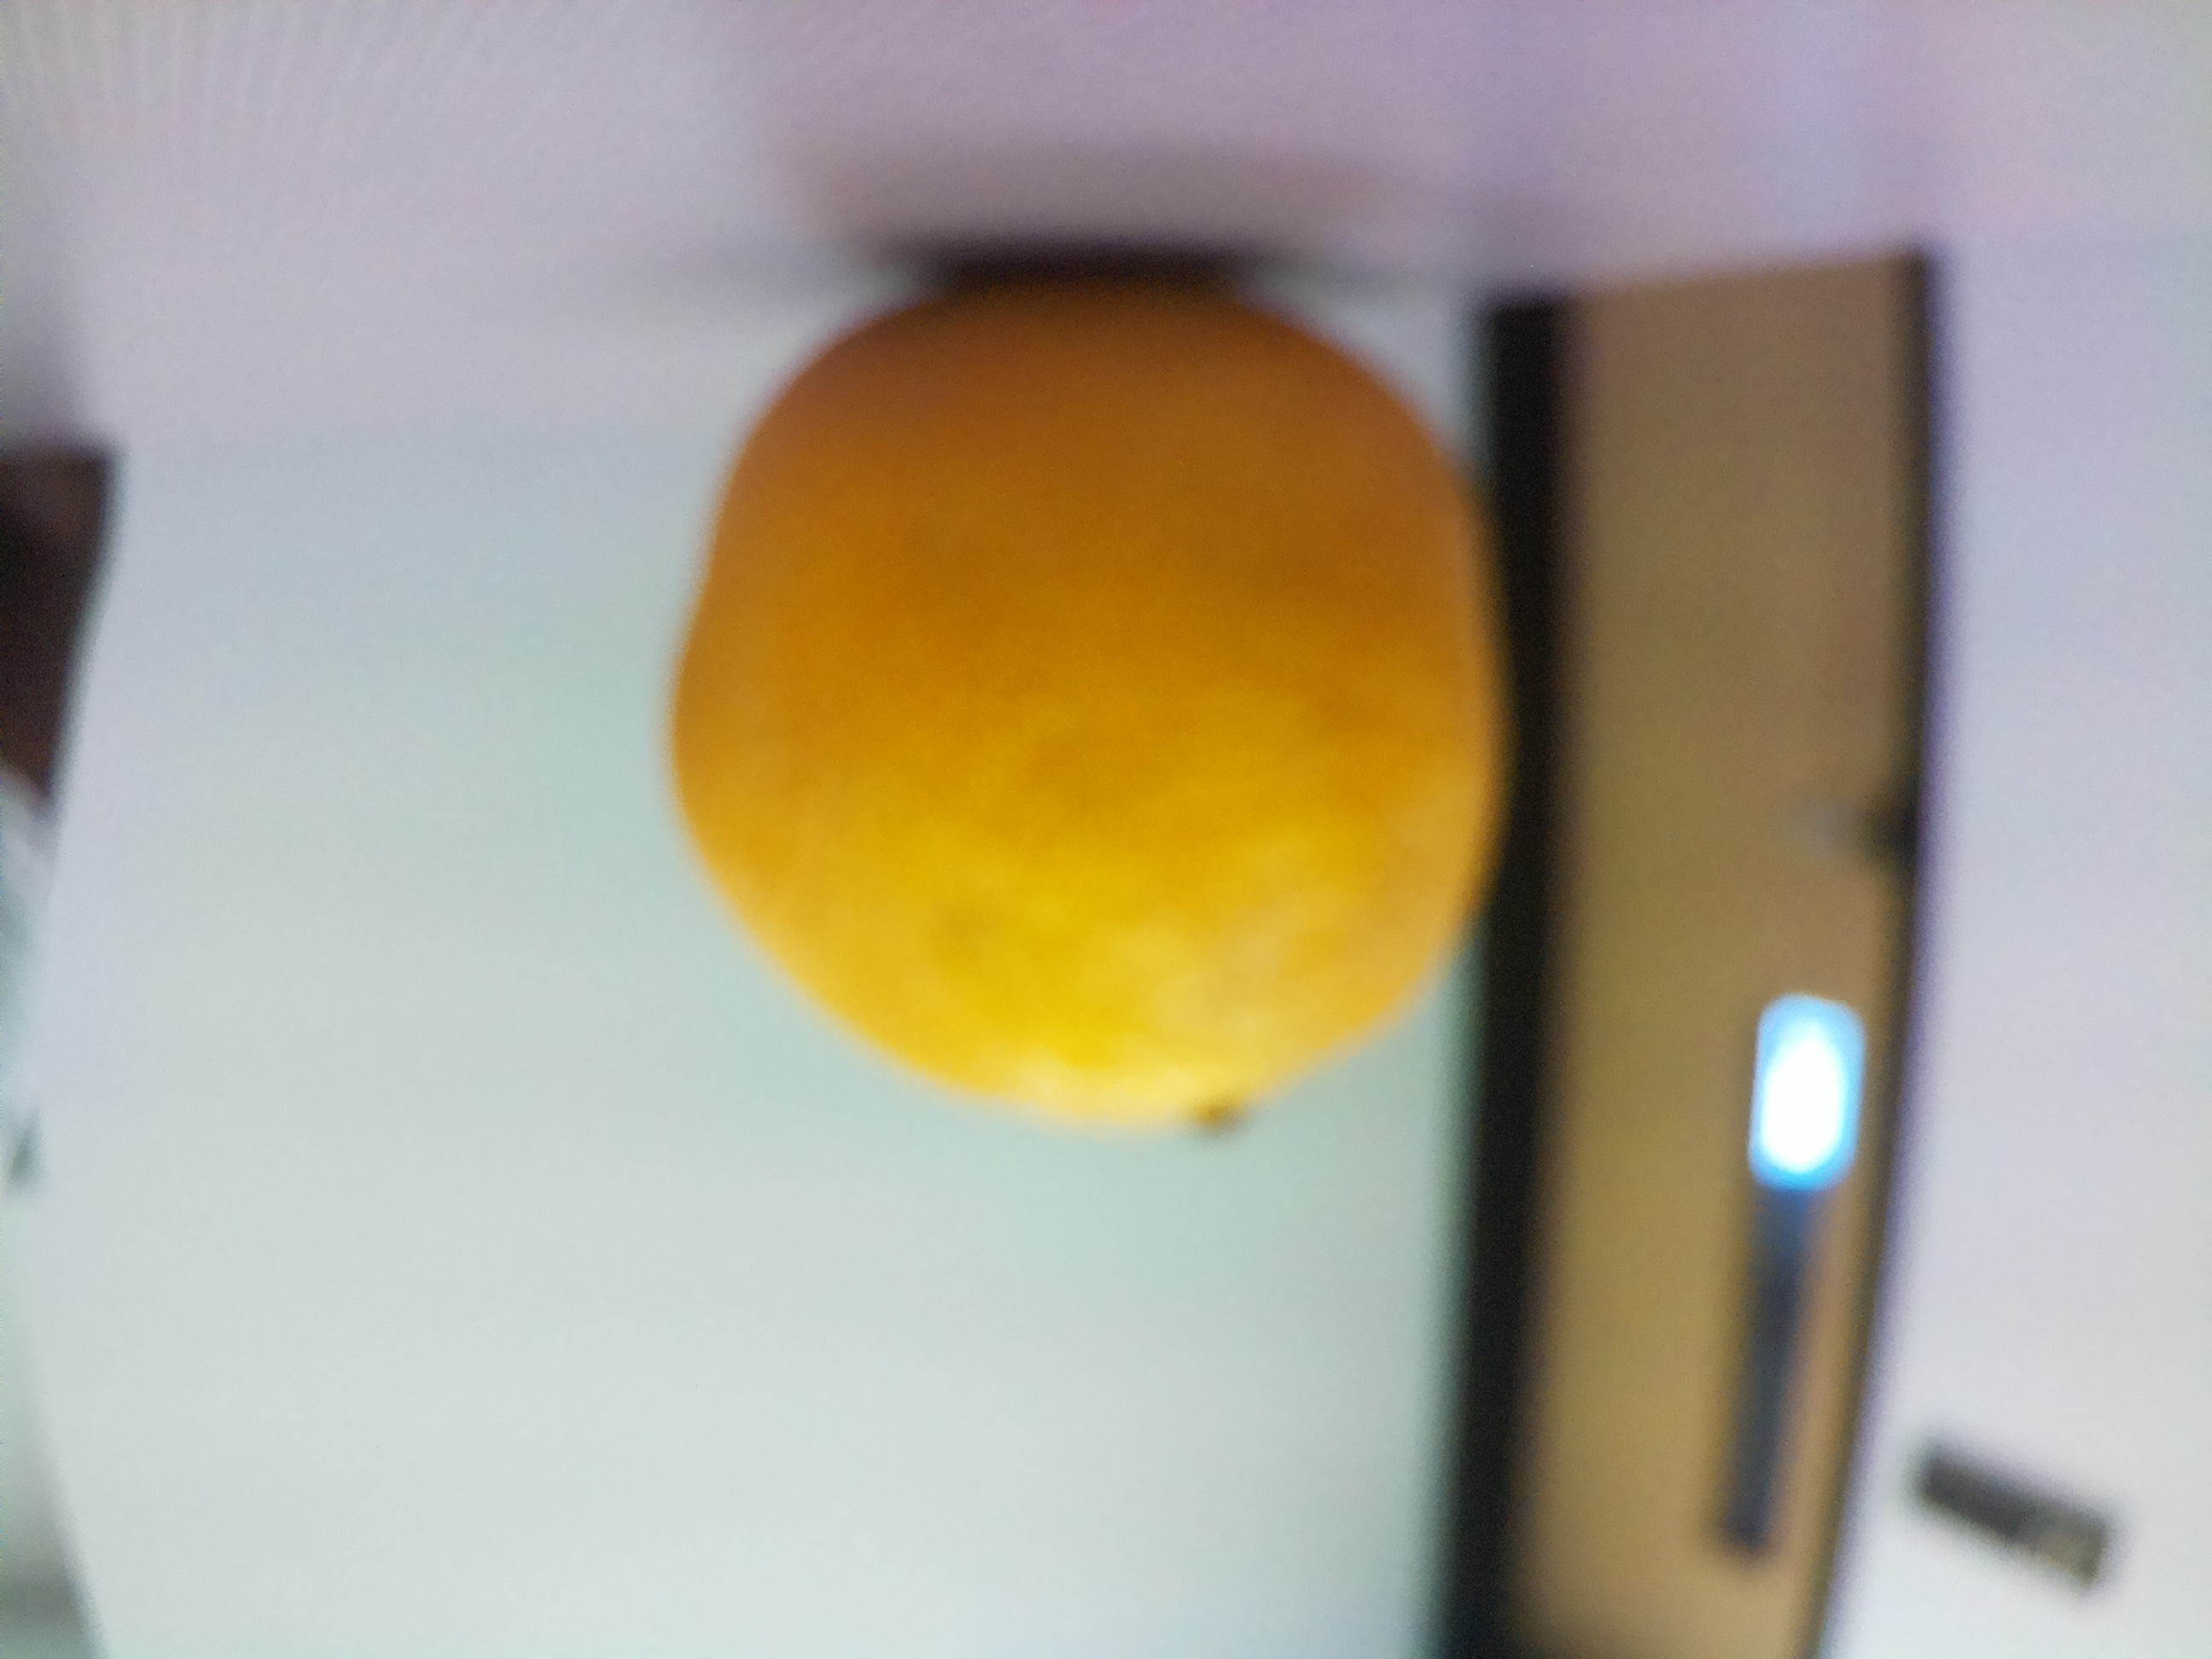
\includegraphics[width=\linewidth, angle=180]{97.png}
        \caption{Image for a Orange}
        \label{fig:image1}
    \end{subfigure}
    \hfill
    \begin{subfigure}{0.3\textwidth}
        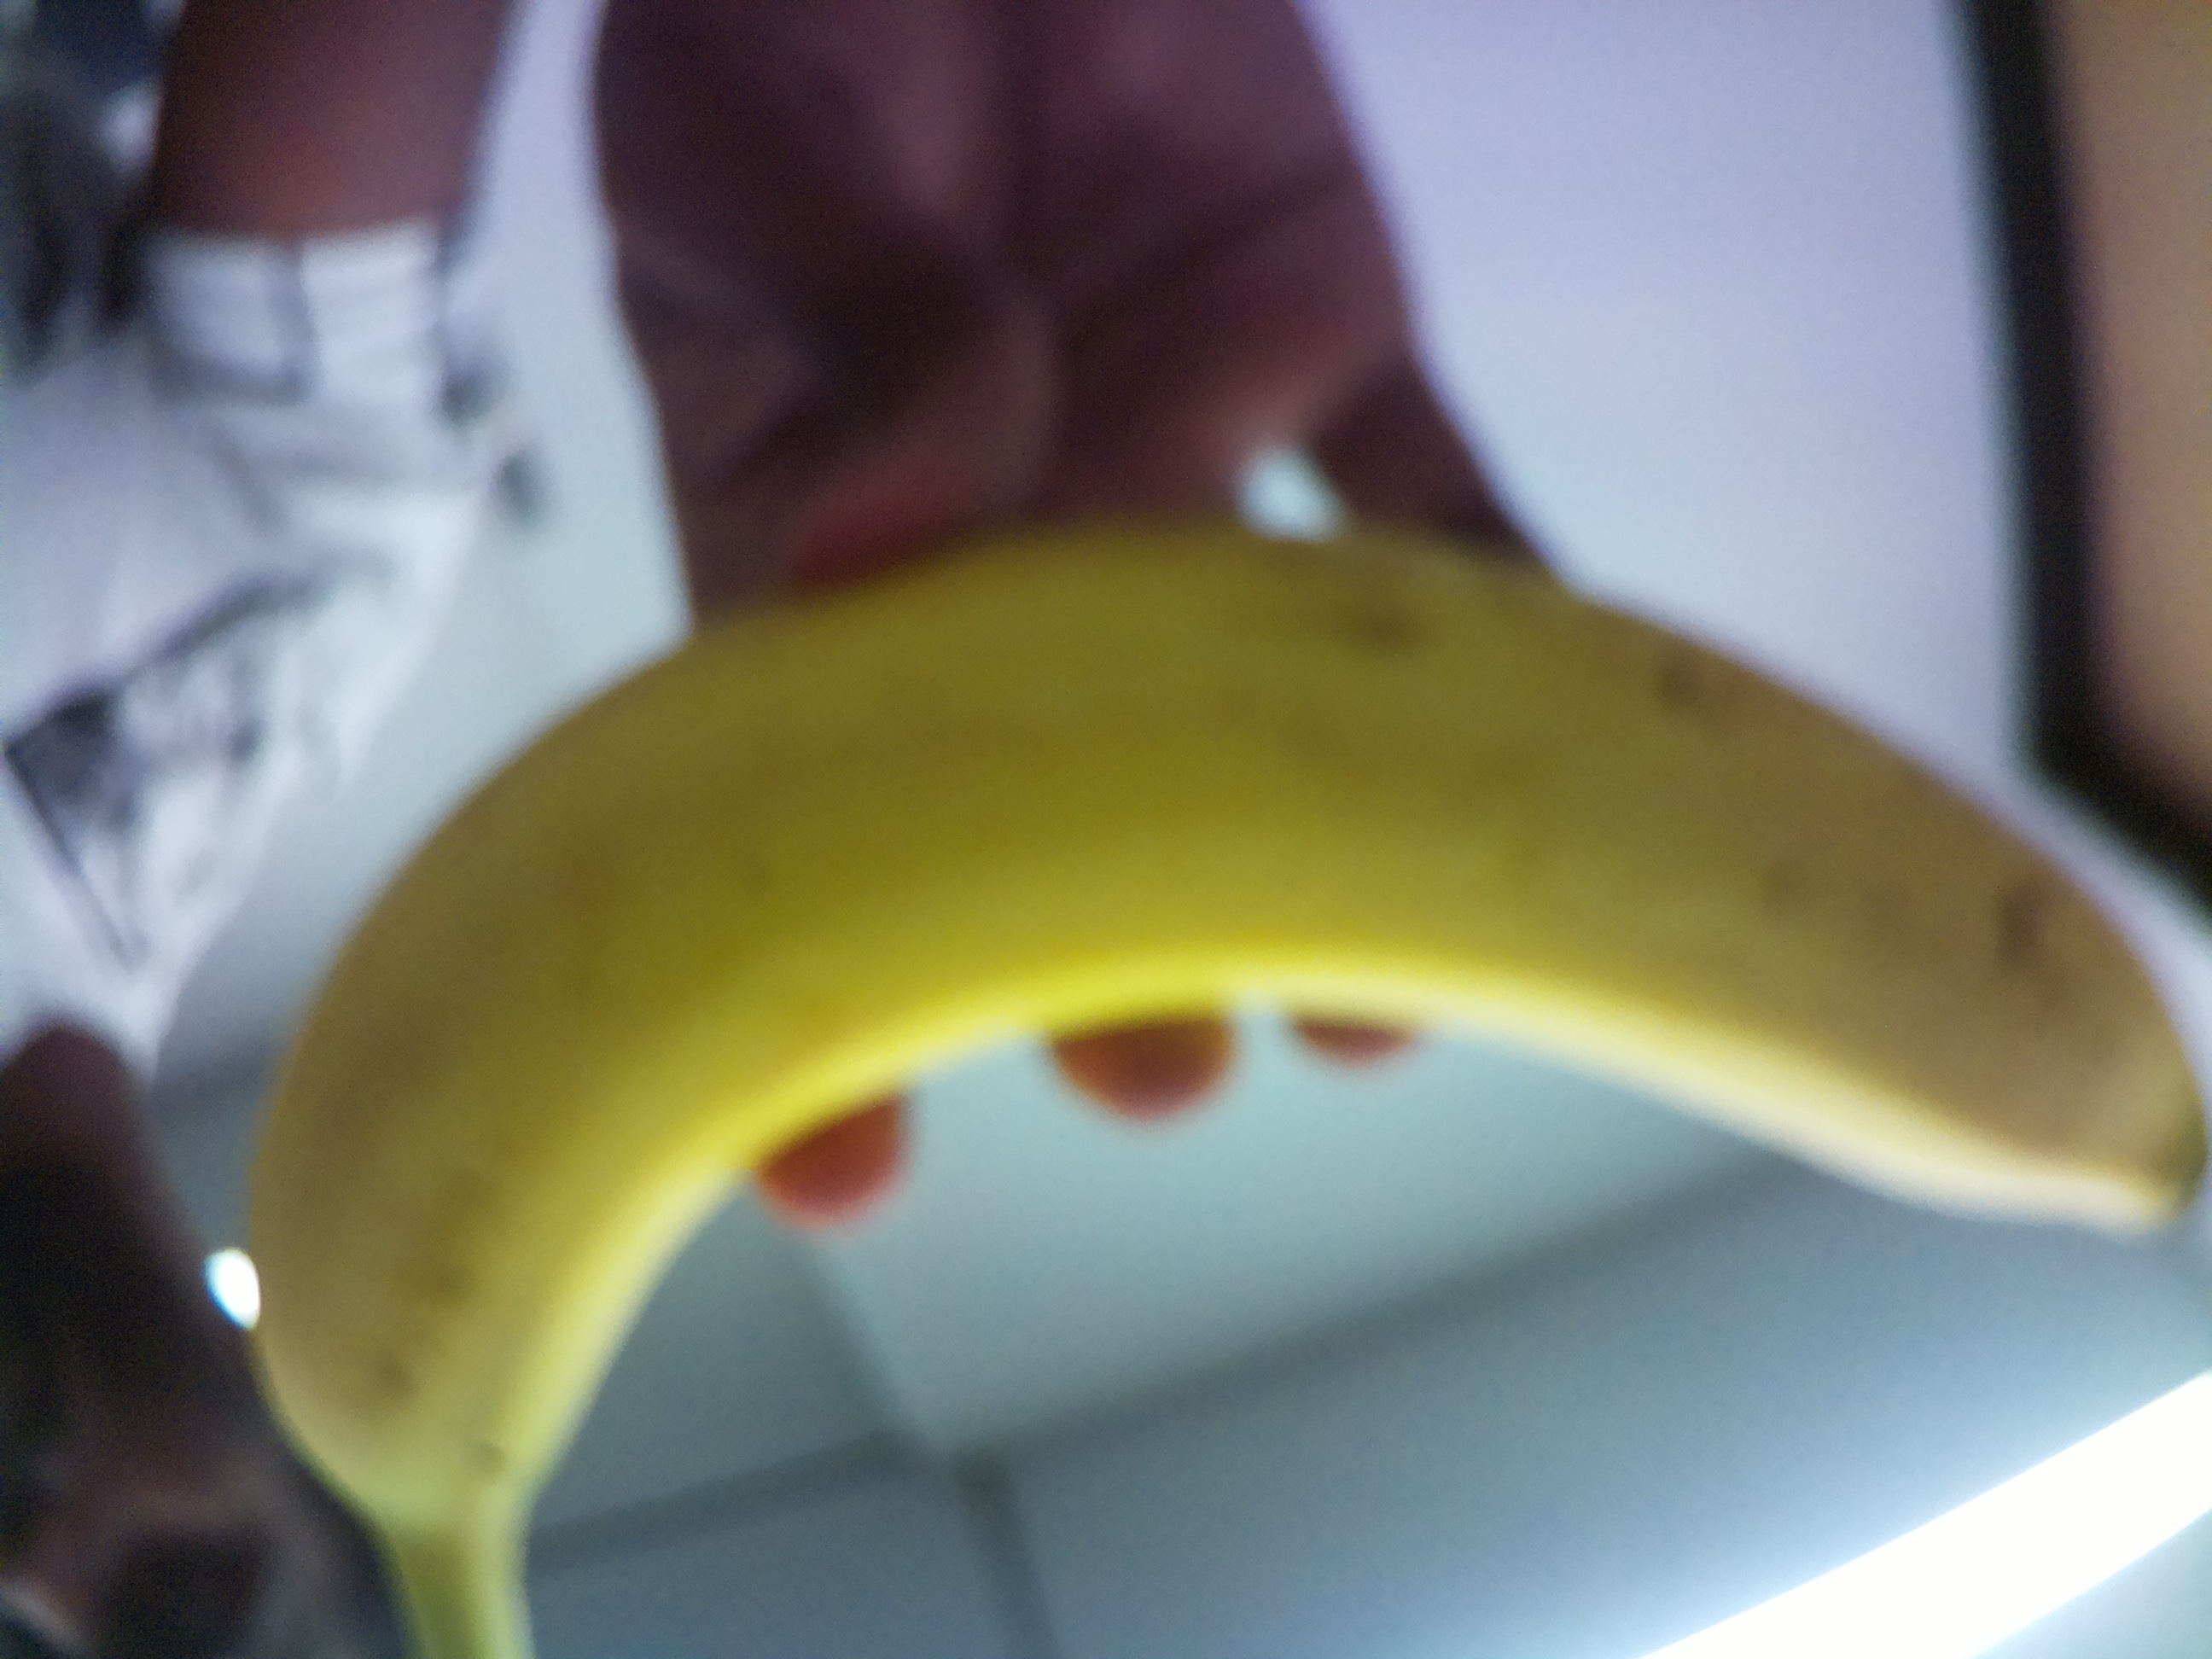
\includegraphics[width=\linewidth, angle = 180]{16.png}
        \caption{Image of an Banana}
        \label{fig:image2}
    \end{subfigure}
    \hfill
    \begin{subfigure}{0.3\textwidth}
        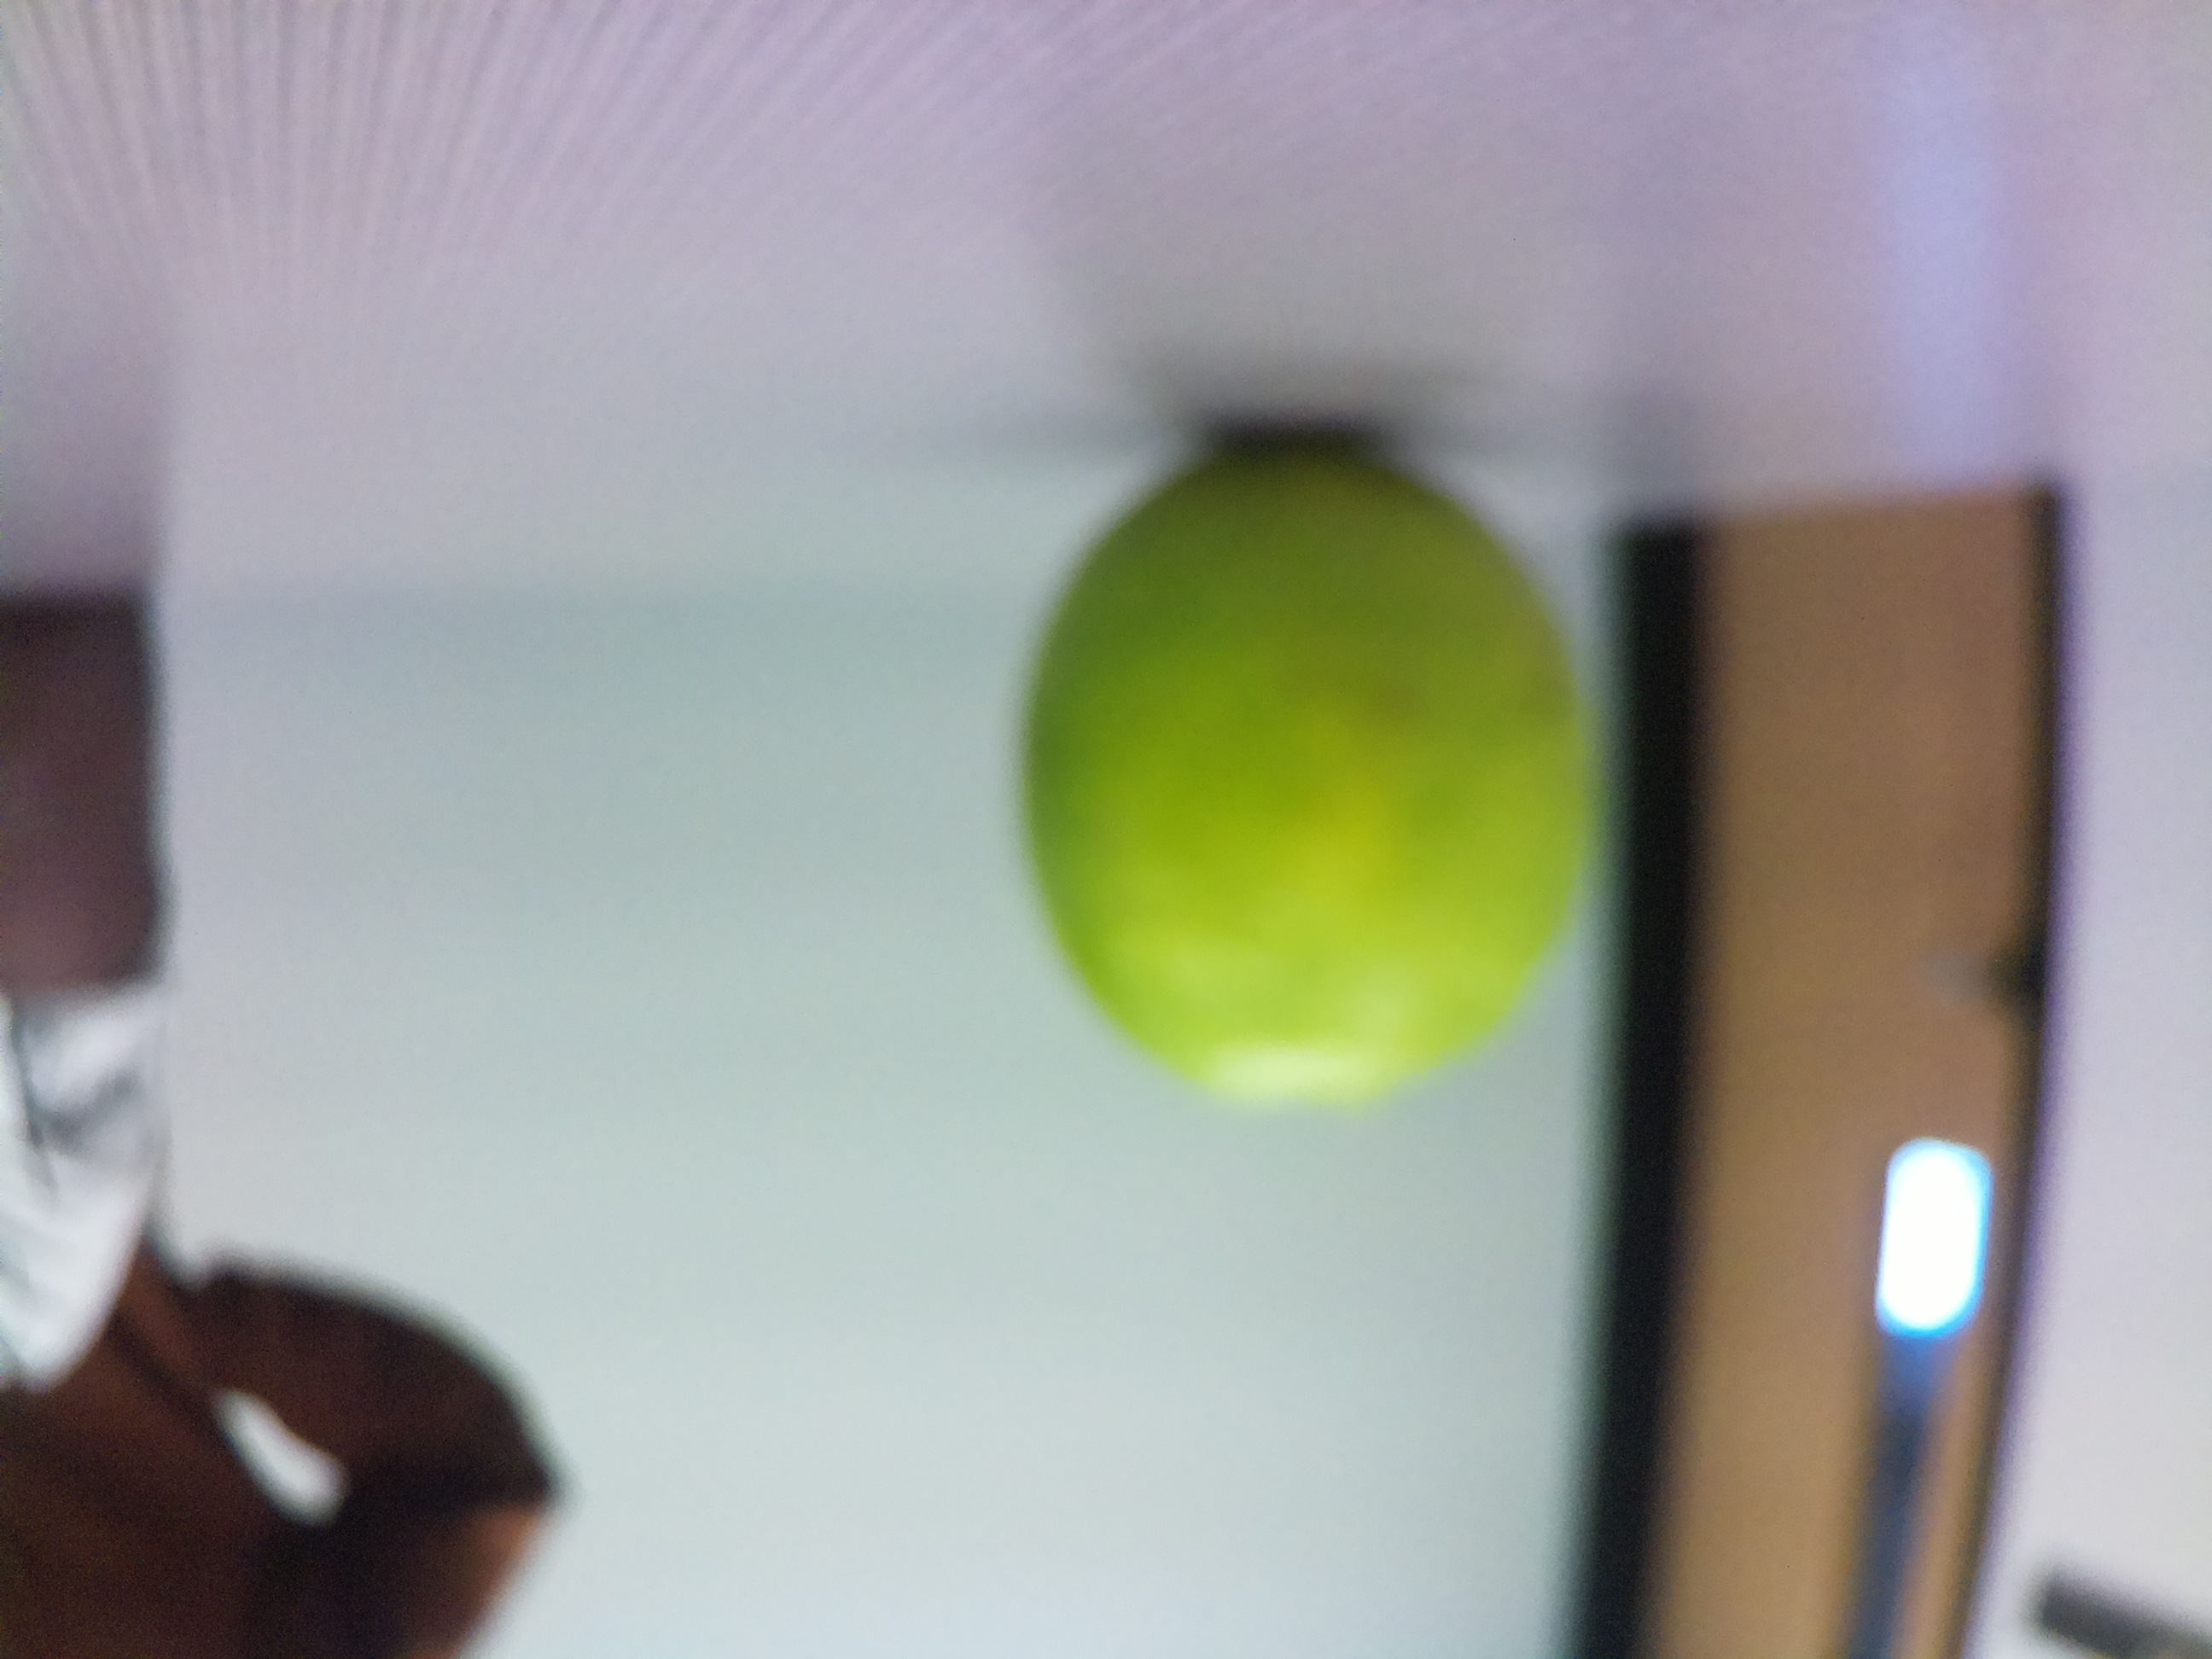
\includegraphics[width=\linewidth, angle = 180]{9.png}
        \caption{Image of a Lime}
        \label{fig:image3}
    \end{subfigure}
    \caption{Images collected through the camera module}
    \label{fig:three_images}
\end{figure}

About more than 200 samples of images of each fruit was collected using the camera module in different environments. Extra data was collected from online scrapping of relevant images which were augmented to our image data which was collected from the micro processor and camera module.

 \vspace{12pt}

\textbf{Convolution Neural Network Model Architecture}

 For image identification, our system utilizes a Convolution Neural Network Model architecture tailored for Raspberry Pi 3b+. While exact details may vary based on the specific machine learning model chosen, the architecture encompasses training the model on a diverse dataset of fruit images, ensuring adaptability to various fruit types and appearances.

The machine learning model is optimized for real-time execution on the Raspberry Pi 3b+, considering the device's computational constraints. Model optimization techniques, such as quantization and compression, may be employed to achieve a balance between accuracy and speed.

From previous work on convolutional neural networks for vision applications we see that depth wise separable convolution are light weight on memory and can be used in light weight embedded systems. The depth wise separable convolution are a subset of the convolution operation where the convolution operation consists of reduced number of parameters. This reduction in parameters allows the neural network to be able to deploy on light weight devices.

\vspace{60pt} 

\textbf{User Interface:}


\begin{figure}[ht]
    \centering
    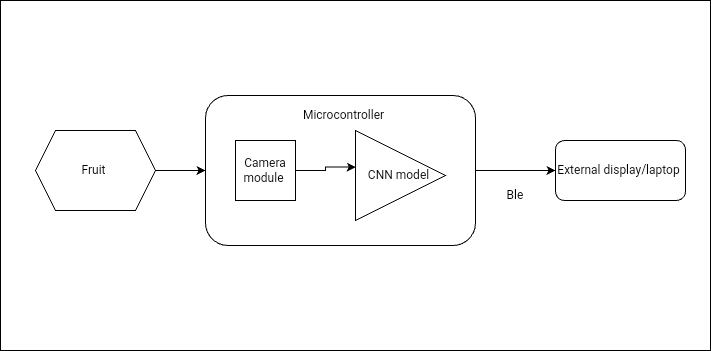
\includegraphics[width=1\linewidth]{Embedded machine learning deployment .drawio.png}
    \caption{System design for Real-Time inference of the machine learning model on Microprocessor}
    \label{fig:2}
\end{figure}
 

\textbf{System Workflow:}

When a shopper places a fruit on the self-checkout counter, the Raspberry camera module v1..0 captures an image of the fruit. Simultaneously, the Raspberry Pi takes in the trained model and runs the real time inference and give the predicted class output on the terminal..

\vspace{12pt} 

\textbf{Real-Time Execution and Model Optimization:}

Ensuring real-time execution is paramount for a smooth self-checkout process. Our system incorporates model optimization techniques to tailor the machine learning model for efficient execution on the Raspberry Pi 3b+. This may involve trade-offs between model accuracy and computational efficiency to meet the real-time constraints of the self-checkout environment.

The comprehensive system design presented here integrates hardware, machine learning, and other components to address the challenges of fruit identification at self-checkout counters. Through the thoughtful combination of these elements, our solution aims to provide an accessible, efficient, and inclusive self-checkout experience for shoppers of all abilities.


\vspace{22pt} 

\section{Evaluation Approach} \label{sec:cite}

Our comprehensive evaluation approach adopts a systematic analysis framework to assess the effectiveness of automated fruit recognition. The primary objectives of our evaluation strategy include quantifying accuracy, efficiency, and inclusivity of the implemented system. The evaluation process is meticulously structured to encompass various critical aspects, covering data collection, model performance metrics, and considerations for user accessibility.

\begin{figure}
    \centering
    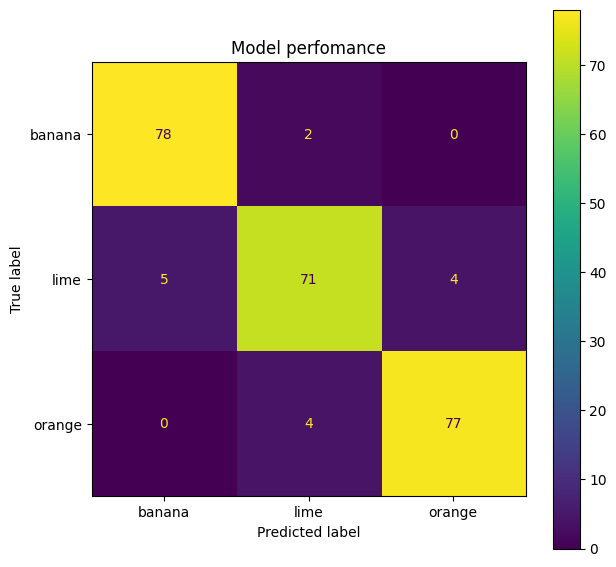
\includegraphics[width=0.75\linewidth]{Untitled.png}
    \caption{Confusion matrix of the test set}
    \label{fig:3}
\end{figure}

The first phase of our evaluation involves an offline assessment conducted during the training of the image recognition model. In this stage, we subject image samples to rigorous testing outside the embedded system environment. By evaluating the model's performance on diverse datasets, we aim to gauge its accuracy, generalization capabilities, and resilience to variations in fruit appearances. This offline evaluation provides insights into the model's foundational robustness and its potential to handle real-world scenarios

The second phase, an online evaluation, takes place after the integration of all components into the microprocessor. This phase aims to validate the model's performance in real-time scenarios within the embedded system. By presenting recognized objects in front of the Raspberry Pi camera module, we assess the accuracy of predictions in a dynamic environment. This process simulates real-world self-checkout scenarios, ensuring the reliability and practical applicability of the automated fruit recognition system.

\begin{figure}
    \centering
    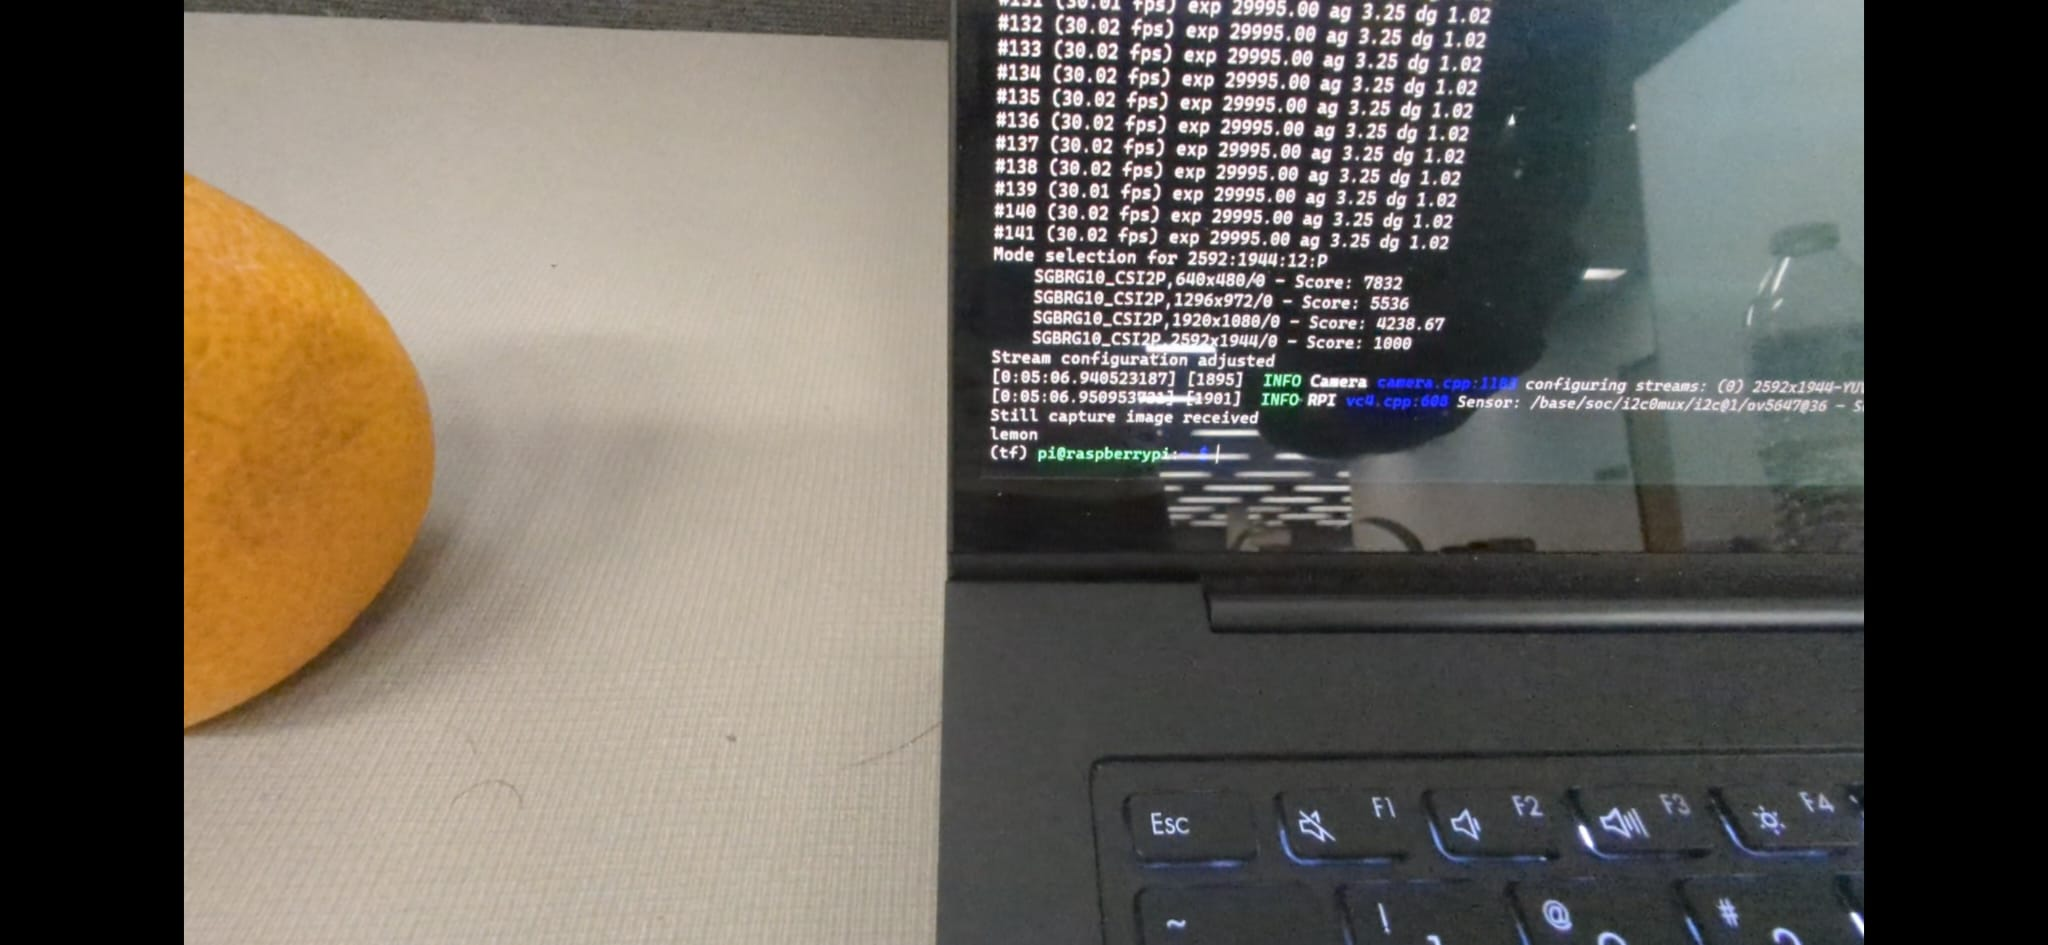
\includegraphics[width=1\linewidth]{WhatsApp Image 2023-12-06 at 21.41.31_e8397d78.jpg}
    \caption{model output when inferenced from raspberry pi}
    \label{fig:4}
\end{figure}

To ensure the robustness and adaptability of the model, the online evaluation incorporates experiments in multiple environments. By exposing the system to diverse  background settings, and fruit arrangements, we validate the model's ability to generalize across various scenarios. This step is crucial for assessing the system's reliability in real-world supermarket environments, where conditions may vary.

In summary, our evaluation approach combines both offline and online assessments, offering a holistic understanding of the automated fruit recognition system's performance. 


\end{document}
